\PassOptionsToPackage{hyphens}{url}
\documentclass[11pt,a4paper]{article}

\usepackage[utf8]{inputenc}
\usepackage[spanish,es-nodecimaldot,es-tabla]{babel}
\usepackage[T1]{fontenc}
\usepackage{lmodern}
\usepackage[margin=2.35cm]{geometry}
\usepackage{amsmath}
\usepackage{amssymb}
\usepackage{booktabs}
\usepackage{longtable}
\usepackage{tabularx}
\usepackage{array}
\usepackage{enumitem}
\usepackage{listings}
\usepackage{xcolor}
\usepackage{microtype}
\usepackage{parskip}
\usepackage{titlesec}
\usepackage{hyperref}
\usepackage{graphicx}
\usepackage{caption}
\usepackage{float}
\usepackage{tocloft}
\setlength{\cftsecnumwidth}{2.2em}
\setlength{\cftsubsecnumwidth}{2.8em}

\definecolor{azulWCD}{RGB}{17,67,112}
\definecolor{grisCodigo}{RGB}{247,247,247}
\definecolor{tituloColor}{RGB}{0,55,110}
\definecolor{reglaColor}{RGB}{0,90,160}

\hypersetup{colorlinks=true, linkcolor=azulWCD, urlcolor=azulWCD, citecolor=azulWCD,
  pdftitle={Validación numérica del modelo WCD con neutrones de 500 MeV}, pdfauthor={Jaime A. Betancourt}}

\lstdefinestyle{shstyle}{backgroundcolor=\color{grisCodigo}, basicstyle=\ttfamily\footnotesize, breaklines=true,
  frame=single, rulecolor=\color{gray!40}, columns=fullflexible, keepspaces=true}
\lstset{style=shstyle}

\titleformat{\section}{\normalfont\Large\bfseries\color{azulWCD}}{\thesection.}{0.6em}{}
\titleformat{\subsection}{\normalfont\large\bfseries}{\thesubsection.}{0.5em}{}
\setlist{itemsep=0.25em,topsep=0.4em}
\renewcommand{\arraystretch}{1.18}
\setlength{\emergencystretch}{2em}
\captionsetup{font=small,labelfont=bf}
\renewcommand{\cftsecfont}{\bfseries\color{azulWCD}}
\renewcommand{\cftsecpagefont}{\bfseries}

\graphicspath{{../figuras/}}
\newcommand{\tablas}{tablas}
\usepackage{url}
\DeclareUrlCommand\archivo{\urlstyle{tt}}
\newcommand{\var}[1]{\texttt{#1}}

\begin{document}
\pagestyle{empty}

\begin{titlepage}
\begin{center}
\vspace*{0.5cm}
\textcolor{reglaColor}{\rule{\linewidth}{1.2pt}}

\vspace{1.3cm}
{\Large\scshape Universidad Industrial de Santander}\\[0.2cm]
{\large Escuela de Física --- Facultad de Ciencias}\\[0.2cm]
{\large Doctorado en Física}

\vspace{2.2cm}
{\Huge\bfseries\color{tituloColor} Validación numérica\\[0.3cm] del modelo WCD con\\[0.3cm] neutrones de 500~MeV}

\vspace{1.2cm}
{\Large Reproducción de Sidelnik et al. (2020) y verificación de la Sección~4.1.1}

\vspace{1.4cm}
{\large\textbf{Informe técnico}}

\vspace{0.6cm}
\begin{minipage}{0.82\linewidth}
\centering
\textit{``Espectros de fotones y electrones, distribución de carga y validación cuantitativa frente a la referencia: procesamiento reproducible, verificación de las cifras de la tesis y pruebas de robustez''}
\end{minipage}

\vfill
{\large\textbf{Autor}}\\[0.15cm]
Jaime A. Betancourt\\[0.1cm]
Doctorado en Física, Universidad Industrial de Santander

\vspace{1.2cm}
\textcolor{reglaColor}{\rule{0.5\linewidth}{0.6pt}}

\vspace{1cm}
9 de octubre de 2026

\vspace{1cm}
\textcolor{reglaColor}{\rule{\linewidth}{1.2pt}}
\end{center}
\end{titlepage}

\pagestyle{plain}

\begin{abstract}
La Sección~4.1.1 de la tesis valida el modelo Monte Carlo del WCD reproduciendo la simulación de Sidelnik et al. (2020), en la que un tanque de 1~m$^3$ con agua pura y con NaCl se irradia con neutrones de 500~MeV. Este informe procesa de forma reproducible los archivos de esa simulación: la carga de seis medios (agua pura y 0.5, 1, 2.5, 5 y 10~\% de NaCl) y los espectros de fotones y electrones de cuatro. Se simularon $2\times10^5$ neutrones por medio, y los conteos absolutos se presentan normalizados a $1.5\times10^5$ neutrones incidentes. Con estos datos el informe verifica las cifras de la sección y prueba la robustez de la validación cuantitativa. Las 15 métricas de la tabla de validación y los 40 parámetros de la tabla de ajustes se reproducen exactamente. Las pruebas, sin embargo, muestran cinco problemas que cambian las conclusiones:
(i)~los $p$-valores ($10^{-77}$--$10^{-175}$) se calcularon sobre 700 puntos interpolados de curvas que tienen 36 bins; con los bins reales $p$ vale $10^{-4}$--$10^{-9}$, y con bins de 25~pe hasta 0.035;
(ii)~la digitalización de la figura de referencia capturó la leyenda como si fuera curva, lo que reduce un 23~\% la razón media de referencia del 2.5~\% de NaCl;
(iii)~la correlación de Pearson no distingue concentraciones: la simulación con 10~\% de NaCl correlaciona mejor con la referencia del 2.5~\% ($r=0.93$) que la propia simulación del 2.5~\% ($r=0.81$);
(iv)~la amplitud de la razón simulada es un 30~\% menor que la de referencia para 2.5 y 5~\% de NaCl;
(v)~en la corrida conservada, los archivos de electrones rotulados 2.5, 5 y 10~\% corresponden en realidad a 5, 10 y 5~\% (el de 2.5 y el de 10~\% son el mismo archivo), y no hay electrones de 2.5~\%; la figura de electrones de la tesis procede del análisis original y no puede verificarse.
La concordancia cualitativa sí se confirma: la razón NaCl/agua pura es menor que 1 por debajo de $\sim$100~pe, la cruza hacia 100--110~pe, alcanza su máximo hacia 290--310~pe y crece de forma ordenada con la concentración.
\end{abstract}

\tableofcontents

% =====================================================================
\section{Objeto y alcance}

La Sección~4.1.1 de la tesis compara el modelo del WCD con el trabajo de Sidelnik et al. (2020) siguiendo la cadena de la señal: captura, fotones gamma, electrones y luz Cherenkov registrada por el PMT. Este informe:
\begin{enumerate}
  \item procesa de forma reproducible los datos de la carpeta \archivo{Seccion-validacion-numerica/Espectros-gamma-500MeV/};
  \item reconstruye cómo se calculó cada cifra de la sección y la verifica;
  \item prueba si la validación cuantitativa resiste cambios razonables de método;
  \item propone correcciones para la tesis.
\end{enumerate}
La distribución de energía de los deuterones (figura \archivo{masa-deuterones-agua-concentraciones-sal} de la tesis) queda pendiente: sus datos no están en la carpeta (Sección~\ref{sec:deuterones}).

\begin{table}[H]
\centering\small
\caption{Correspondencia entre la Sección~4.1.1 de la tesis y este informe.}
\label{tab:correspondencia}
\begin{tabularx}{\linewidth}{@{}>{\raggedright\arraybackslash}p{4.2cm}>{\raggedright\arraybackslash}X>{\raggedright\arraybackslash}p{3.6cm}@{}}
\toprule
\textbf{Tesis} & \textbf{Contenido} & \textbf{Este informe} \\
\midrule
Figs.\ de espectros gamma & Espectro de fotones, cuatro medios, y líneas de captura & Sec.~\ref{sec:gamma} \\
Fig.\ de espectros de electrones & Espectro de electrones frente a la Fig.~5 de la referencia & Sec.~\ref{sec:electrones} \\
Fig.\ de deuterones & Energía de los deuterones de $^1$H(n,$\gamma$) & Sec.~\ref{sec:deuterones} (pendiente) \\
Figs.\ de carga y por tramos & Distribución del número de fotoelectrones & Sec.~\ref{sec:carga} \\
Fig.\ de razones y Tabla de métricas & Validación cuantitativa frente a la referencia digitalizada & Sec.~\ref{sec:validacion} \\
Tabla de ajustes por tramos & Pendientes log--log en cinco intervalos & Sec.~\ref{sec:ajustes} \\
\bottomrule
\end{tabularx}
\end{table}

% =====================================================================
\section{Datos}
\label{sec:datos}

\subsection{Salvedad sobre los datos}
\label{sec:salvedad}

El estudio de validación se realizó originalmente con una simulación de $1.5\times10^5$ neutrones de 500 MeV por medio, cuyos datos se perdieron por un daño del disco. Se conserva una corrida de $2\times10^5$ neutrones por medio, con la que se generaron las figuras y tablas de carga y el espectro gamma de la versión actual de la Sección 4.1.1 (verificado por comparación de archivos y por reproducción exacta de las cifras). No se conservan los datos de la figura de electrones, de la de deuterones ni de las líneas por núcleo; esas figuras corresponden al análisis original.

Este informe analiza la corrida conservada. La Tabla~\ref{tab:fuente} resume qué figuras de la sección se reproducen con ella.

\begin{table}[H]
\centering\small
\caption{Origen de las figuras y tablas de la Sección~4.1.1.}
\label{tab:fuente}
\begin{tabularx}{\linewidth}{@{}>{\raggedright\arraybackslash}p{6.2cm}>{\raggedright\arraybackslash}X@{}}
\toprule
\textbf{Figura o tabla de la tesis} & \textbf{Origen} \\
\midrule
Comparación de histogramas de carga con la referencia & Corrida conservada (figura idéntica píxel a píxel) \\
Razones NaCl/agua pura & Corrida conservada (archivo idéntico) \\
Histograma por intervalos (paneles a--f) & Corrida conservada (archivo idéntico) \\
Tabla de métricas de validación & Corrida conservada (15 cifras reproducidas) \\
Tabla de ajustes por tramos & Corrida conservada (40 valores reproducidos) \\
Espectro gamma de los cuatro medios & Corrida conservada (mismos datos; cambia el tamaño de la imagen) \\
Espectros de electrones & Análisis original (datos no conservados) \\
Energía de los deuterones & Análisis original (datos no conservados) \\
Líneas gamma por núcleo & Análisis original (datos no conservados) \\
\bottomrule
\end{tabularx}
\end{table}

\subsection{Archivos}

La carpeta contiene tres subcarpetas, cada una con los notebooks originales del análisis:
\begin{itemize}
  \item \archivo{Histograma-total-carga/}: un archivo \archivo{Carga\_Total\_Agua\_<medio>\_Neutrones\_500MeV.txt} por medio, con un entero por evento con señal (carga en fotoelectrones, $Q\geq1$). El notebook principal es \archivo{Comparacion\_Histogramas\_Carga.ipynb}; la carpeta incluye además la imagen de la Fig.~6 de la referencia y su digitalización.
  \item \archivo{Espectro-gamma/}: \archivo{Espectro-energia-gamma(s)-<medio>.txt}, una energía en MeV por fila, para agua pura y 2.5, 5 y 10~\% de NaCl.
  \item \archivo{Espectro-electrones/}: \archivo{Espectro-energia-electrones-agua-<medio>[...].txt}, una energía cinética por fila, y dos archivos de partículas secundarias (\archivo{secondary-particles-gamma-compton-*.txt}).
\end{itemize}

\subsection{Qué representa cada fila de los espectros}

Los archivos de partículas secundarias tienen una fila por electrón o positrón creado por un fotón, con el proceso (\var{compt}, \var{phot} o \var{conv}), la posición y tres energías: la del fotón antes de interactuar (columna 9), la del e$^\pm$ (columna 10) y la del fotón después (columna 11). Los archivos de ``gamma'' y de ``electrones'' son, respectivamente, las columnas 9 y 10 de archivos de este tipo. La prueba es directa: emparejados fila a fila, la energía del electrón nunca supera la del fotón (Tabla~\ref{tab:archivos}), mientras que con archivos que no se corresponden eso falla en el 16--17~\% de las filas.

En consecuencia, el ``espectro gamma'' de la tesis no es el espectro de los fotones producidos, sino la \emph{energía del fotón en cada interacción que crea un e$^\pm$}. Un mismo fotón aparece varias veces, una por cada dispersión Compton, con energía decreciente. Por eso la mediana es de solo 86~keV en agua pura, y por eso las líneas de captura aparecen como picos estrechos: corresponden a la primera interacción de fotones que aún no se han dispersado.

\subsection{Normalización y número de eventos}

Se simularon $2\times10^5$ neutrones de 500~MeV por medio. Para compararlos con Sidelnik et al. (2020), todos los conteos absolutos de este informe (tablas y ejes de las figuras) se presentan normalizados a $1.5\times10^5$ neutrones incidentes; los errores estadísticos se calculan con los conteos reales. Las razones NaCl/agua pura, las métricas de validación y las pendientes de los ajustes no dependen de esta normalización.

\begin{table}[H]
\centering\small
\caption{Eventos con señal ($Q\geq1$) por cada $1.5\times10^5$ neutrones incidentes, fracción de neutrones que producen señal ($\varepsilon$) y estadística de la carga por medio.}
\label{tab:carga}
\begin{tabular}{@{}lrrrrrr@{}}
\toprule
Medio & Eventos & $\varepsilon$ (\%) & $\langle Q\rangle$ (pe) & $\sigma_Q$ (pe) & Mediana & Máximo \\
\midrule
\input{\tablas/tabla_carga.tex} \\
\bottomrule
\end{tabular}
\end{table}

Entre el 79.8 y el 80.8~\% de los neutrones producen señal, es decir, entre 119\,702 y 121\,254 eventos por cada $1.5\times10^5$ neutrones. La fracción apenas depende del medio: a 500~MeV la señal la dominan las cascadas hadrónicas y no la captura.

% =====================================================================
\section{Espectros de fotones y líneas de captura}
\label{sec:gamma}

\begin{figure}[H]
\centering
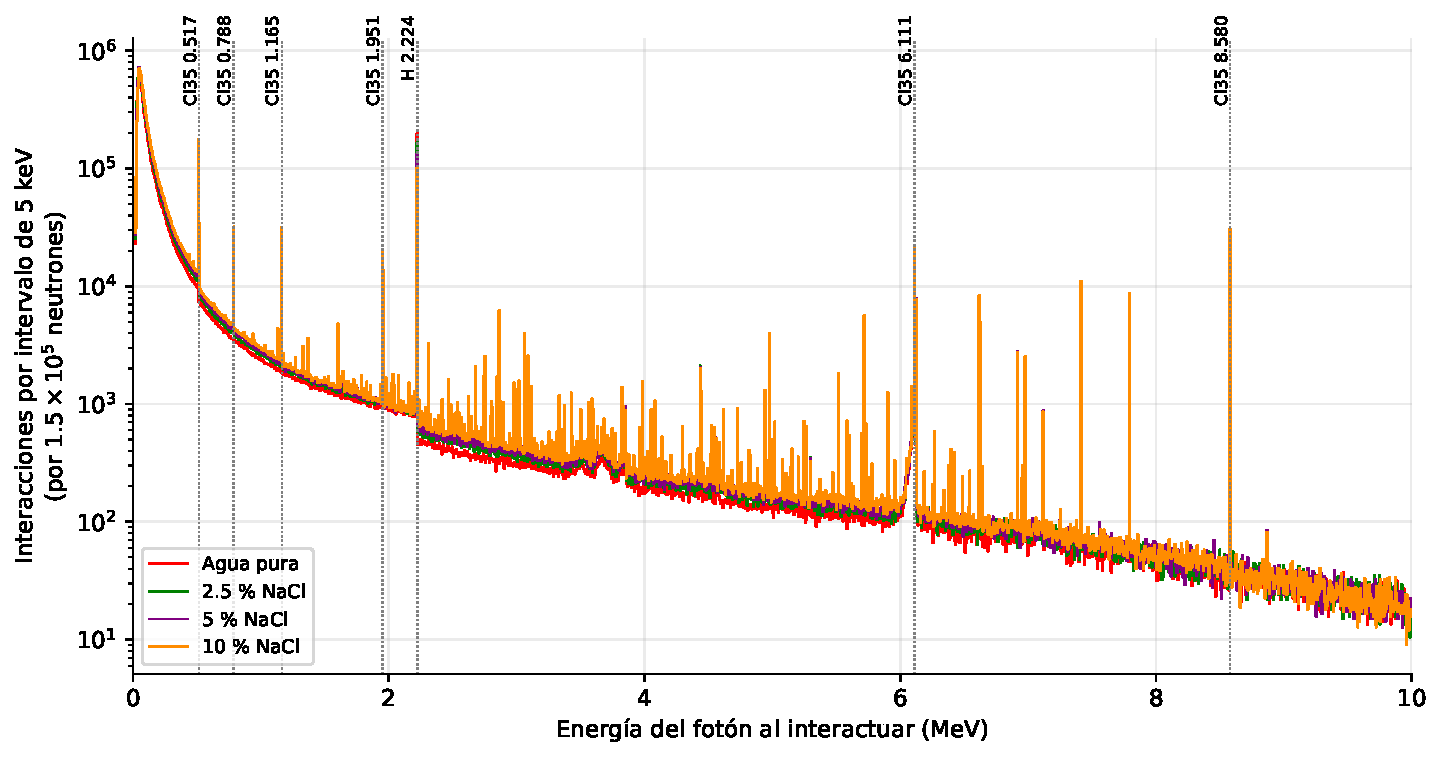
\includegraphics[width=\linewidth]{espectro_gamma.pdf}
\caption{Energía del fotón en cada interacción que crea un e$^\pm$, para los cuatro medios (intervalos de 5~keV). Las líneas punteadas marcan las líneas de captura con la energía que usa Geant4.}
\label{fig:gamma}
\end{figure}

\begin{table}[H]
\centering\small
\caption{Líneas de captura: energía tabulada (NNDC, Tabla de la tesis), energía en Geant4 (valor de 0.01~keV más poblado a $\pm2$~keV) y número de interacciones a $\pm0.05$~keV de ese valor, por cada $1.5\times10^5$ neutrones incidentes.}
\label{tab:lineas}
\begin{tabular}{@{}lrrrrrr@{}}
\toprule
Núcleo & $E_\text{tabla}$ (keV) & $E_\text{Geant4}$ (keV) & Agua pura & 2.5~\% & 5~\% & 10~\% \\
\midrule
\input{\tablas/tabla_lineas.tex} \\
\bottomrule
\end{tabular}
\end{table}

\begin{itemize}
  \item \textbf{Hidrógeno.} La línea aparece a 2224.37~keV, no a 2223.25~keV: G4NDL usa un valor 1.12~keV mayor que el de NNDC. El ajuste de la tesis ($\mu=2.22437$~MeV) es correcto, pero la Tabla de parámetros nucleares lista 2223.25~keV sin advertir la diferencia. Las interacciones de la línea bajan de 197\,552 en agua pura a 100\,144 con 10~\% de NaCl (por cada $1.5\times10^5$ neutrones), porque el cloro compite por la captura.
  \item \textbf{Cloro 35.} Sus líneas crecen con la concentración. La de mayor energía está a 8579.81~keV en Geant4 frente a 8578.6~keV en la tabla. En agua pura las cuentas en esas energías son las del fondo, así que no hay cloro.
  \item \textbf{Oxígeno y cloro 37.} Sus líneas apenas superan el fondo (entre 3 y 400 cuentas por cada $1.5\times10^5$ neutrones, frente a un fondo de 2 a 100), de acuerdo con sus secciones eficaces pequeñas.
\end{itemize}

La comparación con la Fig.~3 de la referencia sigue siendo cualitativa. Para que fuera cuantitativa habría que saber si Sidelnik et al. histogramaron la misma magnitud (energía de interacción o energía de emisión).

% =====================================================================
\section{Espectros de electrones}
\label{sec:electrones}

\begin{table}[H]
\centering\small
\caption{Archivos de electrones: filas, fracción de filas con $E_e\leq E_\gamma$ frente al archivo de fotones con el que mejor se emparejan, medio real y suma MD5 (primeros 8 caracteres).}
\label{tab:archivos}
\begin{tabular}{@{}lrrll@{}}
\toprule
Archivo & Filas & $E_e\leq E_\gamma$ & Medio real & MD5 \\
\midrule
\input{\tablas/tabla_archivos_electrones.tex} \\
\bottomrule
\end{tabular}
\end{table}

El emparejamiento identifica el medio de cada archivo de electrones:
\begin{itemize}
  \item \archivo{…agua-pura.txt} corresponde a agua pura;
  \item \archivo{…agua-25NaCl.txt} corresponde a la corrida de \textbf{5~\%};
  \item \archivo{…agua-5NaCl.txt} corresponde a la de \textbf{10~\%};
  \item \archivo{…agua-10NaCl-1.txt} es \textbf{idéntico} (misma MD5) a \archivo{…agua-25NaCl.txt}, es decir, también 5~\%;
  \item \archivo{…agua-10NaCl.txt} y los dos archivos \archivo{-Meiga} no se emparejan con ningún archivo de fotones: vienen de otras corridas.
\end{itemize}
No hay ningún archivo de electrones de la corrida de 2.5~\% que acompañe a los espectros de fotones.

\begin{figure}[H]
\centering
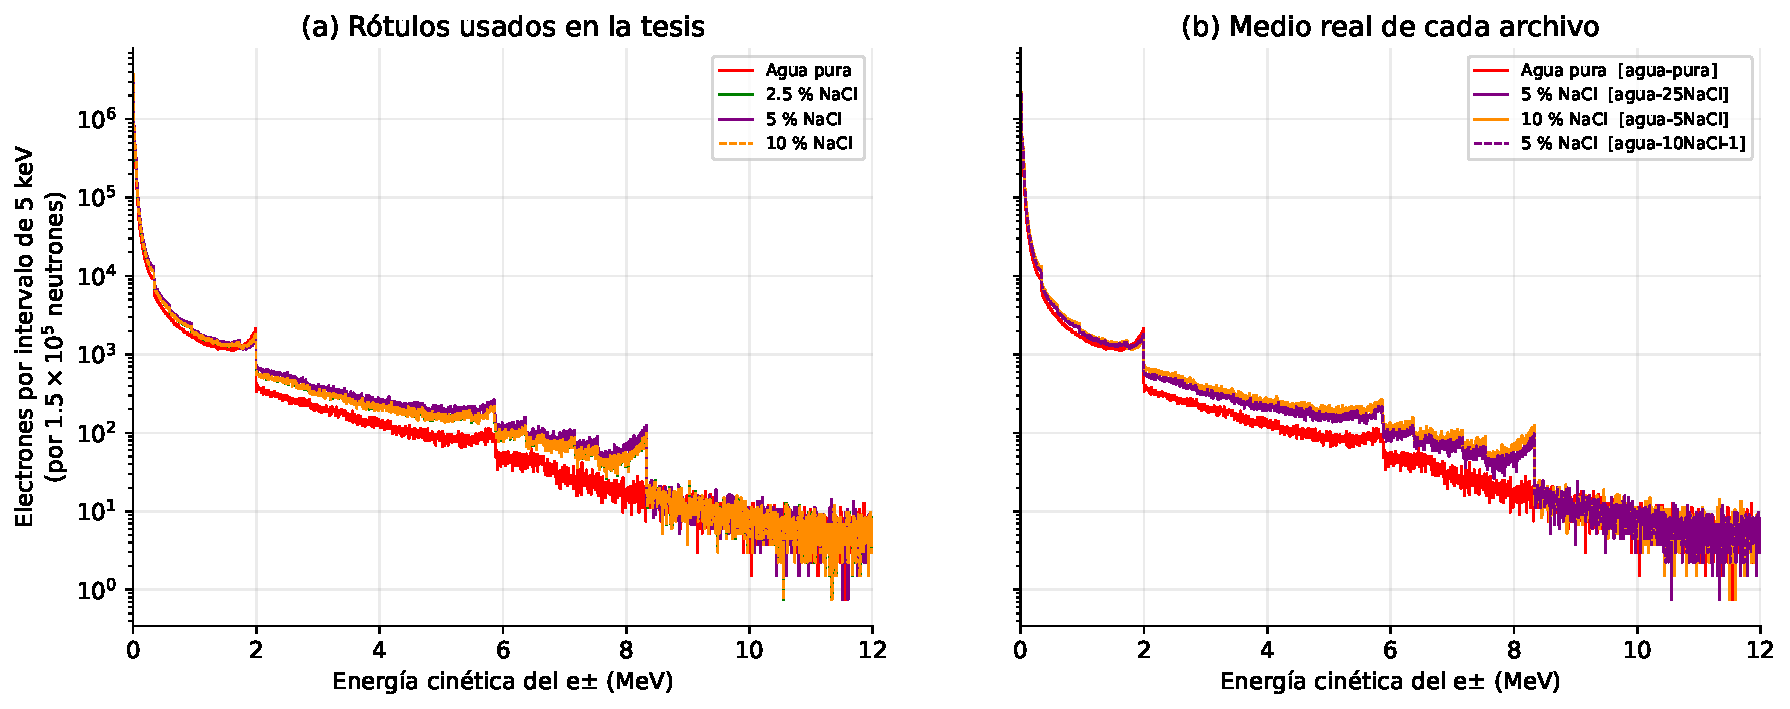
\includegraphics[width=\linewidth]{espectro_electrones.pdf}
\caption{Espectros de electrones de la corrida conservada, con los archivos que usa el notebook original. (a) Con los rótulos de los nombres de archivo: la curva verde (2.5~\%) queda oculta bajo la naranja (10~\%) porque son el mismo archivo. (b) Con el medio real de cada archivo.}
\label{fig:electrones}
\end{figure}

El notebook de la carpeta (\archivo{Analisis-Espectro-Electrones.ipynb}) dibuja \archivo{pura}, \archivo{25NaCl}, \archivo{5NaCl} y \archivo{10NaCl-1}; con la corrida conservada, sus curvas de 2.5, 5 y 10~\% son en realidad 5, 10 y 5~\%. La figura de electrones de la tesis no es esa: tiene cuatro curvas distintas y ninguna combinación de los archivos conservados la reproduce, de modo que procede del análisis original (Sección~\ref{sec:salvedad}). Los bordes Compton que discute el texto (1.994~MeV para la línea del H y $\sim$8.35~MeV para la de 8.58~MeV del cloro) sí aparecen en los datos conservados (Fig.~\ref{fig:electrones}).

% =====================================================================
\section{Distribución de la carga}
\label{sec:carga}

\begin{figure}[H]
\centering
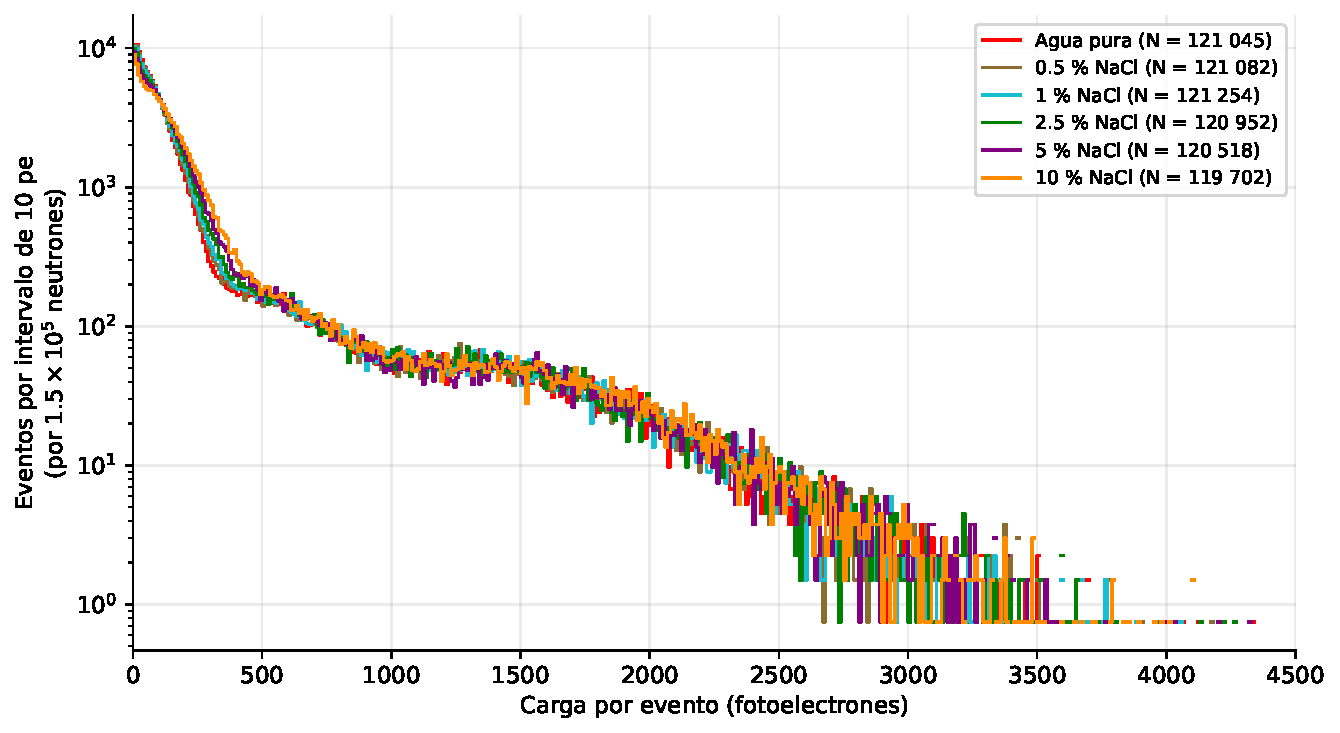
\includegraphics[width=0.9\linewidth]{histograma_carga.pdf}
\caption{Distribución de la carga por evento (intervalos de 10~pe, por cada $1.5\times10^5$ neutrones incidentes) en los seis medios simulados.}
\label{fig:histograma}
\end{figure}

\begin{figure}[H]
\centering
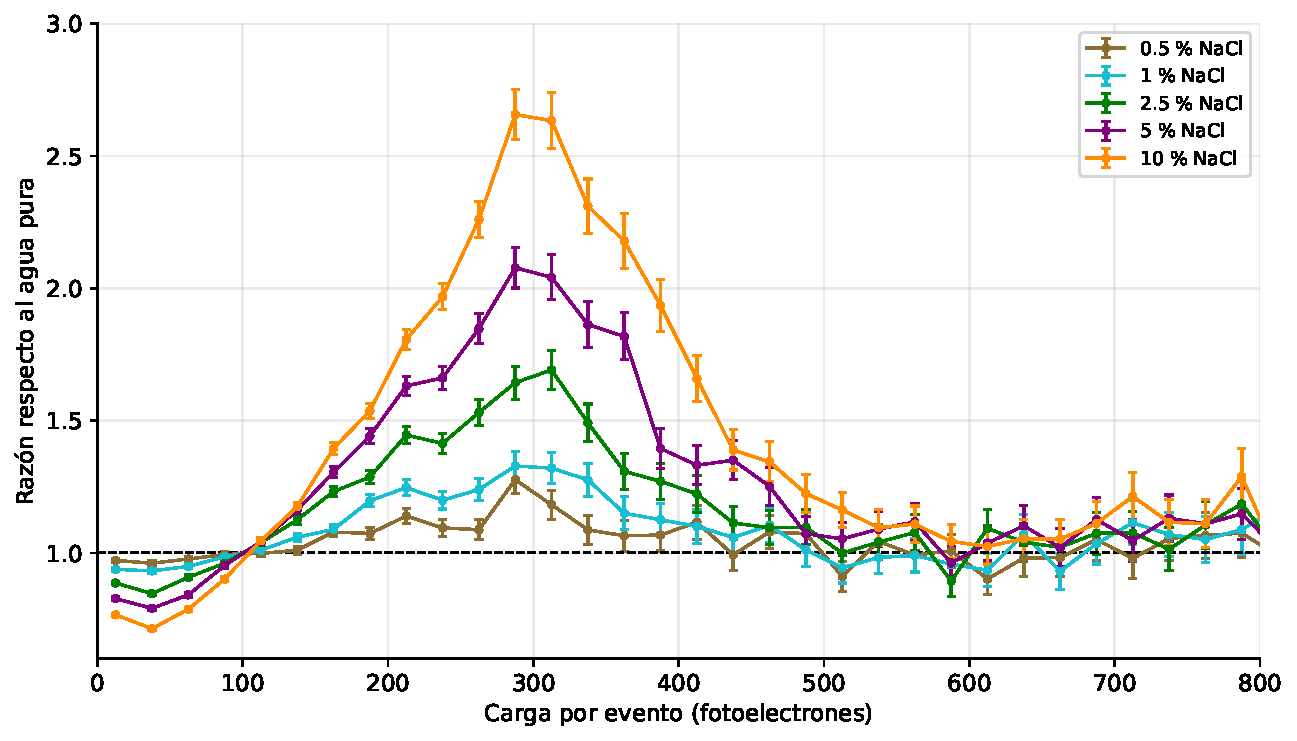
\includegraphics[width=0.9\linewidth]{razon_carga_medios.pdf}
\caption{Razón entre la distribución normalizada de cada medio con NaCl y la del agua pura, en intervalos de 25~pe y sin suavizar, con error de Poisson.}
\label{fig:razon-medios}
\end{figure}

Las afirmaciones cualitativas del texto se confirman sin suavizar y con errores de Poisson (Fig.~\ref{fig:razon-medios}):
\begin{itemize}
  \item la razón es menor que 1 por debajo de $\sim$100~pe, y menor cuanto mayor es la concentración (0.77 para 10~\% a 12~pe);
  \item cruza la unidad hacia 100--110~pe en todos los medios;
  \item crece hasta un máximo hacia 290--310~pe: $1.69\pm0.07$ (2.5~\%), $2.08\pm0.08$ (5~\%) y $2.66\pm0.09$ (10~\%);
  \item vuelve a $\sim$1 hacia 500~pe; la tesis dice ``450'';
  \item mantiene el orden $10>5>2.5$~\%. Las corridas de 0.5 y 1~\%, que la tesis no usa, encajan en la misma secuencia.
\end{itemize}
Solo el 0.2~\% de los eventos supera 2500~pe. El texto describe el histograma ``hasta 6000 fotones'', pero el máximo registrado es de 4640~pe.

% =====================================================================
\section{Validación cuantitativa frente a la referencia}
\label{sec:validacion}

\subsection{Método original}

El notebook original calcula las razones así:
\begin{enumerate}
  \item histogramas de 300 intervalos en 0--2500 (8.3~pe cada uno), normalizados por su suma;
  \item suavizado con una media móvil de 5 intervalos;
  \item razón NaCl/agua pura.
\end{enumerate}
La referencia se obtiene digitalizando la imagen de la Fig.~6 de Sidelnik et al.:
\begin{enumerate}
  \item máscaras de color por curva;
  \item mediana vertical de los píxeles de cada columna;
  \item malla de 700 puntos, normalizada por el área en 0--2500.
\end{enumerate}
Las métricas se calculan sobre 700 puntos interpolados entre 100 y 400~pe. Con ese método se reproducen exactamente las 15 cifras de la tesis (Tabla~\ref{tab:metricas}).

\begin{table}[H]
\centering\small
\caption{Métricas de validación: valor de la tesis / valor recalculado con el método original.}
\label{tab:metricas}
\begin{tabular}{@{}lccccc@{}}
\toprule
Medio & $r$ & $p$ & $\rho$ & RMSE & MAE \\
\midrule
\input{\tablas/tabla_metricas.tex} \\
\bottomrule
\end{tabular}
\end{table}

\subsection{Problemas}

\paragraph{1. Los $p$-valores.} Los 700 puntos no son independientes: salen de interpolar 36 intervalos simulados (y la referencia, de una curva dibujada). El test de Pearson supone 698 grados de libertad cuando hay como mucho 34, lo que reduce artificialmente el $p$-valor en más de cien órdenes de magnitud. Con los intervalos reales, $p$ queda entre $10^{-9}$ y $10^{-4}$, y con intervalos de 25~pe sube a 0.035 para el 10~\% (Tabla~\ref{tab:variantes}).

\paragraph{2. Los artefactos de la digitalización.} Las máscaras de color capturaron las líneas de la leyenda de la figura original como si fueran curva: hay picos de hasta 5000 cuentas entre 1550 y 1850~pe en las curvas de 2.5 y 5~\% (Fig.~\ref{fig:artefactos}), y un punto anómalo en 0~pe. Los picos quedan fuera de la ventana de 100--400~pe, pero entran en el área con la que se normaliza toda la curva. Al reemplazarlos por interpolación, la razón media de referencia en 100--400~pe sube de 1.50 a 1.94 (2.5~\%) y de 1.99 a 2.20 (5~\%); la del 10~\% casi no cambia (1.90 frente a 1.91). Con la referencia corregida, el RMSE del 2.5~\% pasa de 0.25 a 0.65, y el ``mejor acuerdo'' que la tesis atribuye al 2.5~\% desaparece.

\begin{figure}[H]
\centering
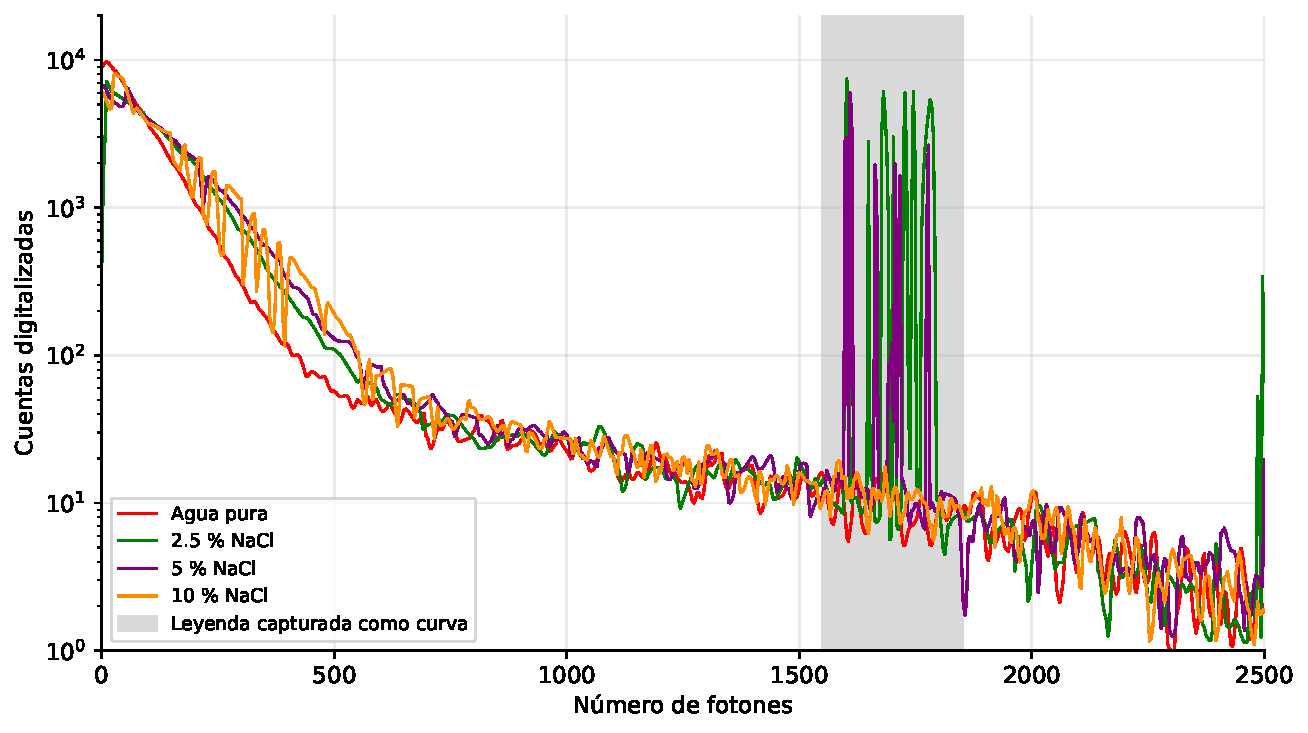
\includegraphics[width=0.85\linewidth]{digitalizacion_artefactos.pdf}
\caption{Curvas digitalizadas de la Fig.~6 de Sidelnik et al. La franja gris marca los picos producidos por la leyenda.}
\label{fig:artefactos}
\end{figure}

\paragraph{3. Pearson no mide el acuerdo.} En 100--400~pe todas las razones suben y luego bajan, así que cualquier par de curvas correlaciona. Para comprobarlo se calculó $r$ entre cada una de las cinco simulaciones y cada curva de referencia (Fig.~\ref{fig:control}a). Frente a la referencia del 2.5~\%, la simulación que más correlaciona es la del 10~\% ($r=0.93$), no la del 2.5~\% ($r=0.81$). Frente a la del 10~\%, la que más correlaciona es la del 0.5~\% ($r=0.75$). El coeficiente no distingue la concentración y no sirve como prueba de validación.

\begin{figure}[H]
\centering
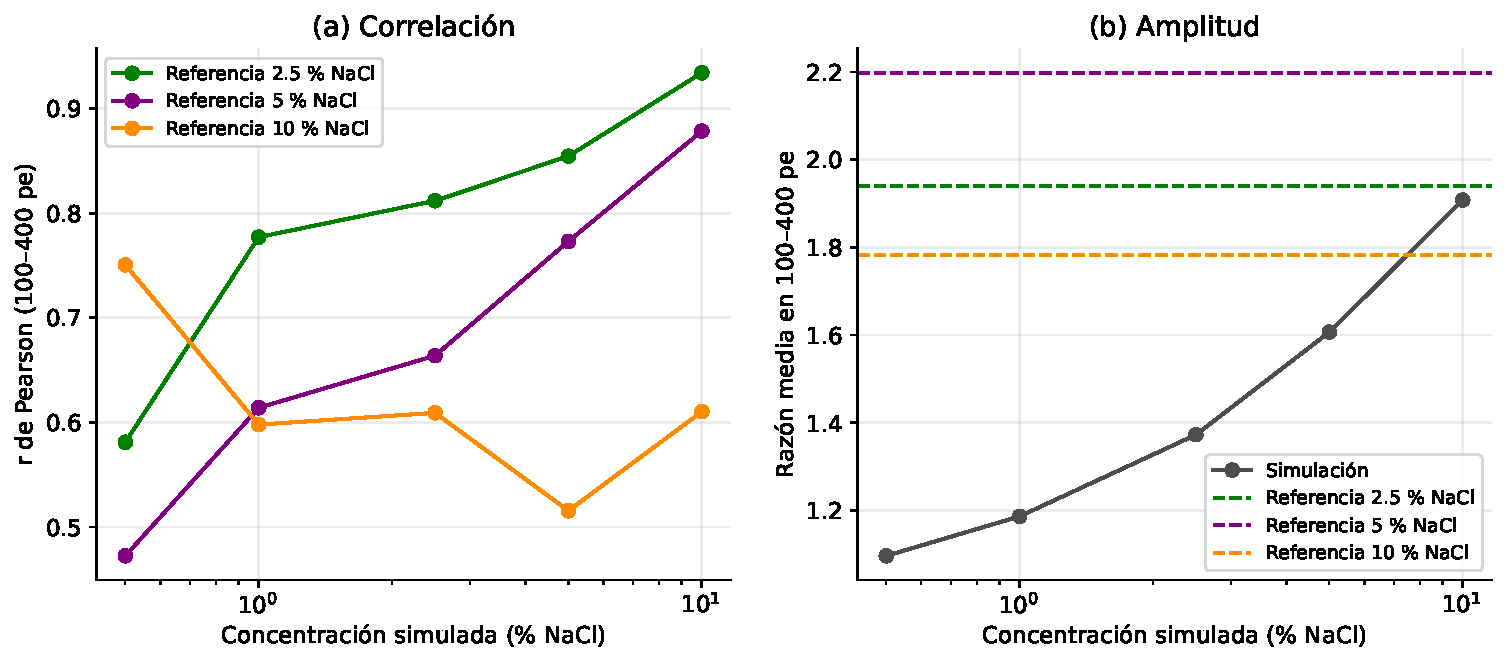
\includegraphics[width=\linewidth]{control_pearson.pdf}
\caption{(a) Correlación de Pearson entre cada simulación y cada curva de referencia (sin artefactos), en 100--400~pe y con intervalos de 25~pe. (b) Razón media en 100--400~pe: simulación (gris) y referencias (líneas discontinuas).}
\label{fig:control}
\end{figure}

\paragraph{4. La amplitud.} Lo que sí distingue la concentración es la amplitud de la razón (Fig.~\ref{fig:control}b): la razón media simulada crece de forma monótona de 1.10 (0.5~\%) a 1.91 (10~\%). Frente a la referencia corregida, la simulación queda un 29~\% por debajo para el 2.5~\% (1.37 frente a 1.94) y un 27~\% para el 5~\% (1.61 frente a 2.20); para el 10~\% coincide (1.91 frente a 1.78), aunque esa curva de referencia es muy ruidosa porque la original es punteada. Los máximos simulados están en 290--310~pe; los de referencia, en 318~pe (2.5~\%) y 383~pe (5 y 10~\%). Además, por encima de $\sim$350~pe la razón simulada vuelve a 1 antes que la de referencia (Fig.~\ref{fig:sim-ref}).

\begin{figure}[H]
\centering
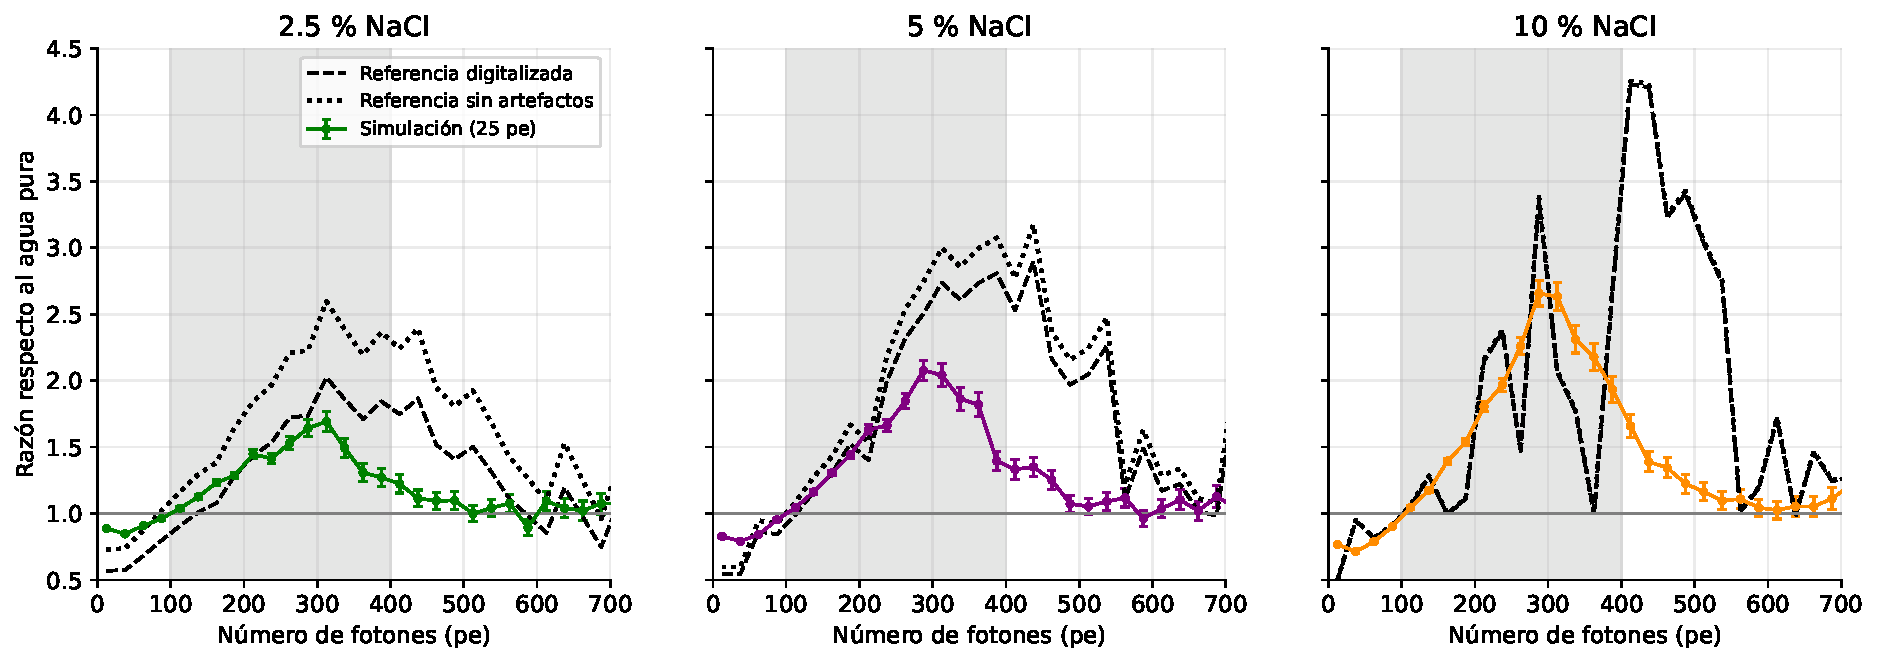
\includegraphics[width=\linewidth]{razon_simulacion_referencia.pdf}
\caption{Razón simulada (intervalos de 25~pe, error de Poisson) frente a la digitalizada de la referencia, cruda (discontinua) y sin artefactos (punteada). La franja gris es la ventana de las métricas de la tesis.}
\label{fig:sim-ref}
\end{figure}

\paragraph{5. El suavizado.} La media móvil reduce el ruido de la razón simulada y sube $r$ (0.72 frente a 0.82 en el 2.5~\%), pero no cambia la amplitud. No es un error, pero debe declararse.

{\small\setlength{\tabcolsep}{4pt}
\begin{longtable}{@{}llrrrrrr@{}}
\caption{Métricas de validación con distintas variantes del método. $n$: puntos usados; $\bar R$: razón media en 100--400~pe de la simulación y de la referencia.}
\label{tab:variantes}\\
\toprule
Variante & Medio & $n$ & $r$ & $p$ & RMSE & $\bar R_\text{sim}$ & $\bar R_\text{ref}$ \\
\midrule
\endfirsthead
\toprule
Variante & Medio & $n$ & $r$ & $p$ & RMSE & $\bar R_\text{sim}$ & $\bar R_\text{ref}$ \\
\midrule
\endhead
\input{\tablas/tabla_variantes.tex} \\
\bottomrule
\end{longtable}}

\subsection{Lectura}

La simulación reproduce la \emph{forma} de la respuesta: la razón es menor que 1 a baja carga, cruza la unidad hacia 100~pe, tiene un máximo y se ordena con la concentración. No reproduce la \emph{amplitud} de la referencia para 2.5 y 5~\%: el efecto del NaCl es un 30~\% menor. Las causas posibles son las que la tesis ya menciona (versión de Geant4, G4NDL, óptica y eficiencia cuántica), a las que se suma la incertidumbre de la digitalización. La validación debería presentarse como una concordancia cualitativa con una diferencia de amplitud cuantificada, no como una correlación estadísticamente significativa.

% =====================================================================
\section{Ajustes por tramos}
\label{sec:ajustes}

La tabla de ajustes de la tesis reúne pendientes e interceptos de rectas ajustadas a $(\log_{10}Q,\log_{10}N)$ en cinco tramos. El ajuste es log--log, es decir, una ley de potencias $N\propto Q^{a}$, aunque el texto lo describe como ``escala semi-log'' y habla de ``caída exponencial''. Se reconstruyó el origen de cada cifra probando nueve binnings (Tabla~\ref{tab:ajustes}):
\begin{itemize}
  \item \textbf{Binning A} (400 intervalos en 0--6000, 15~pe): da los valores de 0--100, 100--500 y 500--1000. El tramo ``0--100'' es en realidad 10--100~pe, con solo 6 puntos.
  \item \textbf{Binning B} (200 intervalos en 0--6000, 30~pe; celda 34 del notebook): da los valores de 1000--1500 y 1500--3500, y los \emph{errores} de 100--500 y 500--1000. En esos dos tramos la tesis combina el valor de un ajuste con el error de otro.
  \item Los errores de 0--100 ($\pm0.010$--$0.015$) no salen de ninguno de los binnings probados.
\end{itemize}

Además, el ajuste por mínimos cuadrados sobre $\log_{10}N$ descarta los intervalos vacíos y da el mismo peso a todos, lo que sesga la pendiente donde hay pocas cuentas. Un ajuste de máxima verosimilitud de Poisson, con intervalos de 10~pe que incluyen los vacíos, cambia sobre todo el último tramo: $-4.4\pm0.08$ en los cuatro medios, frente a $-5.4$ a $-5.7$ en la tesis (Fig.~\ref{fig:ajustes}). En 100--500~pe muestra una tendencia clara con la sal ($-2.41$ a $-1.90$) que la tesis no recoge, y en 0--100~pe conserva el orden de la tesis con valores algo distintos.

\begin{figure}[H]
\centering
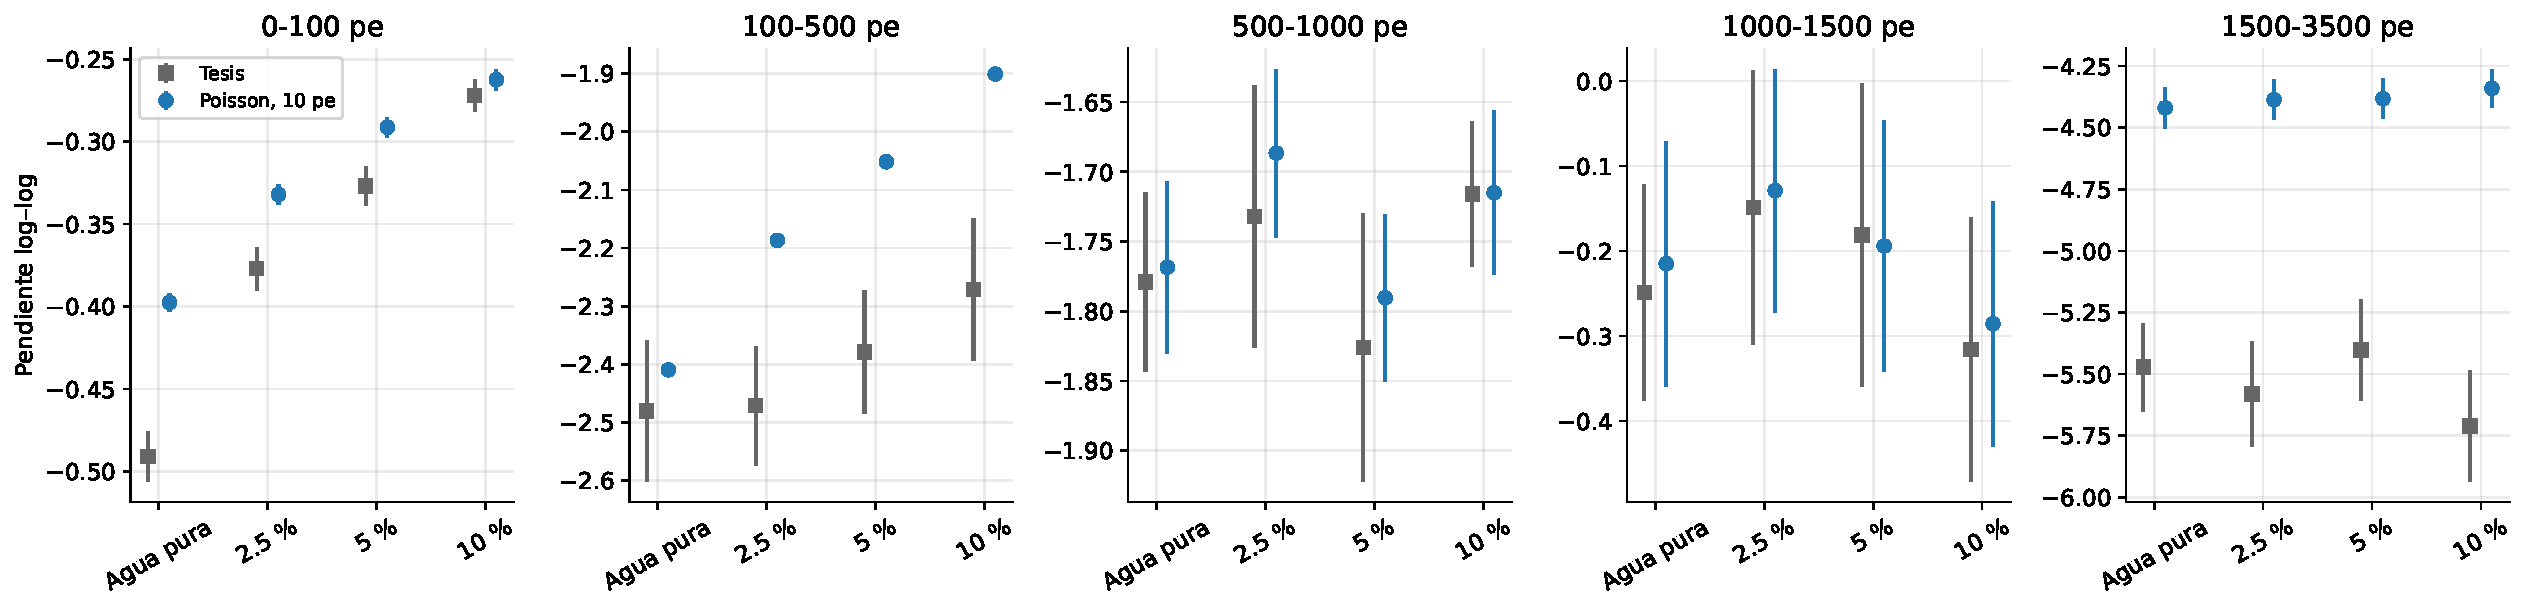
\includegraphics[width=\linewidth]{ajustes_tramos.pdf}
\caption{Pendientes log--log por tramo: tesis (cuadrados) y ajuste de Poisson con intervalos de 10~pe (círculos).}
\label{fig:ajustes}
\end{figure}

{\small\setlength{\tabcolsep}{3.5pt}
\begin{longtable}{@{}llccccc@{}}
\caption{Pendientes de los ajustes por tramos. Origen: binning del que salen el valor y el error de la tesis (A, B, o --- si no se encontró). A y B: ajustes por mínimos cuadrados con cada binning; Poisson: máxima verosimilitud con intervalos de 10~pe.}
\label{tab:ajustes}\\
\toprule
Tramo (pe) & Medio & Tesis & Origen & A & B & Poisson \\
\midrule
\endfirsthead
\toprule
Tramo (pe) & Medio & Tesis & Origen & A & B & Poisson \\
\midrule
\endhead
\input{\tablas/tabla_ajustes.tex} \\
\bottomrule
\end{longtable}}

% =====================================================================
\section{Deuterones (pendiente)}
\label{sec:deuterones}

La figura de deuterones de la tesis (\archivo{Figuras/masa-deuterones-agua-concentraciones-sal.png}) no tiene datos en esta carpeta. El generador \archivo{analysis/figuras-tesis/regenerar\_figuras.py} ya la recalculó en octubre de 2026 desde \archivo{Espectros-500MeV/<medio>/captura-hidrogeno.txt}, pero solo para agua pura y 2.5~\%; su resumen (\archivo{deuterones.tsv}) da un pico en $1.3190\pm0.0101$ y $1.3190\pm0.0104$~keV, igual al valor cinemático $E_\gamma^2/2M_dc^2=1.319$~keV. Si esto se confirma con los cuatro medios, la afirmación de la tesis de que ``el valor medio y el ancho de la distribución aumentan con la concentración de NaCl'' no se sostiene: el pico es el mismo, y lo que cambia es el número de deuterones. El autor está buscando los archivos \archivo{captura-hidrogeno.txt} en su almacenamiento.

% =====================================================================
\section{Correcciones propuestas para la tesis}

\begin{enumerate}
  \item \textbf{Salvedad sobre los datos.} Mencionar en la sección la pérdida de los datos originales de $1.5\times10^5$ neutrones y la corrida conservada de $2\times10^5$ (Sección~\ref{sec:salvedad}).
  \item \textbf{Espectro gamma.} Indicar que es la energía del fotón en cada interacción que crea un e$^\pm$, no el espectro de emisión.
  \item \textbf{Línea del H.} Indicar en la Tabla de parámetros nucleares que Geant4 la sitúa en 2224.37~keV (y la de 8578.6~keV del $^{35}$Cl en 8579.81~keV).
  \item \textbf{Espectros de electrones.} La figura de la tesis procede del análisis original. Si se quisiera regenerar con la corrida conservada, solo hay datos de agua pura, 5 y 10~\%, y hay que usar el medio real de cada archivo (Tabla~\ref{tab:archivos}).
  \item \textbf{Validación cuantitativa.} Sustituir la Tabla de métricas por una comparación de amplitud (razón media y máximo en 100--400~pe, simulación con error de Poisson) con la referencia digitalizada sin artefactos, y retirar los $p$-valores o recalcularlos con los grados de libertad reales. Reescribir el párrafo del ``mejor acuerdo para 2.5~\%'' y la frase ``coincidencia de los parámetros integrales''.
  \item \textbf{Ajustes por tramos.} Rehacer la tabla con un único binning y ajuste de Poisson; corregir ``semi-log'' y ``exponencial'' por ``ley de potencias (log--log)''; cambiar el tramo ``0--100'' por ``10--100''.
  \item \textbf{Texto del histograma.} ``Hasta 6000 fotones'' debe ser ``hasta $\sim$4600~pe''; ``vuelve a la unidad a partir de 450'' debe ser ``hacia 500~pe''.
  \item \textbf{Deuterones.} Revisar la afirmación sobre la media y el ancho cuando estén los datos.
\end{enumerate}

% =====================================================================
\section{Reproducibilidad}

Desde \archivo{analysis/validacion-numerica-Sidelnik\_seccion-4.1.1/}:
\begin{lstlisting}
python3 procesar_500MeV.py <Espectros-gamma-500MeV> resultados    # ~40 s
python3 analizar_validacion.py resultados datos
python3 construir_notebook.py
jupyter nbconvert --to notebook --execute figuras_seccion_4.1.1.ipynb
python3 tablas_informe.py resultados informe/tablas
\end{lstlisting}
\archivo{procesar\_500MeV.py} lee los 3.3~GB de datos crudos y escribe 2~MB de resúmenes. El resto funciona solo con \archivo{resultados/} y con la digitalización de la referencia (\archivo{datos/}).

% =====================================================================
\section{Conclusiones}

\begin{enumerate}
  \item El procesamiento de la simulación de 500~MeV es reproducible, y las 55 cifras de las tablas de métricas y de ajustes de la tesis se recuperan exactamente a partir de los datos crudos.
  \item La simulación reproduce cualitativamente la referencia: razón menor que 1 a baja carga, cruce hacia 100~pe, máximo hacia 300~pe y orden con la concentración. Las líneas de captura del H y del $^{35}$Cl aparecen donde las sitúa Geant4.
  \item La validación cuantitativa de la tesis no resiste las pruebas: los $p$-valores están inflados por la interpolación, la digitalización de la referencia tiene artefactos que sesgan la curva del 2.5~\%, y la correlación de Pearson no distingue concentraciones. La amplitud del efecto del NaCl es un 30~\% menor que en la referencia para 2.5 y 5~\%.
  \item En la corrida conservada, los archivos de electrones están mal rotulados y falta el de 2.5~\%; la figura de electrones de la tesis procede del análisis original.
  \item La tabla de ajustes mezcla dos binnings y un ajuste sesgado en los tramos con pocas cuentas.
  \item Queda pendiente el análisis de los deuterones.
\end{enumerate}
\end{document}
